% mnras_template.tex 
%
% LaTeX template for creating an MNRAS paper
%
% v3.0 released 14 May 2015
% (version numbers match those of mnras.cls)
%
% Copyright (C) Royal Astronomical Society 2015
% Authors:
% Keith T. Smith (Royal Astronomical Society)

% Change log
%
% v3.0 May 2015
%    Renamed to match the new package name
%    Version number matches mnras.cls
%    A few minor tweaks to wording
% v1.0 September 2013
%    Beta testing only - never publicly released
%    First version: a simple (ish) template for creating an MNRAS paper

%%%%%%%%%%%%%%%%%%%%%%%%%%%%%%%%%%%%%%%%%%%%%%%%%%
% Basic setup. Most papers should leave these options alone.
\documentclass[fleqn,usenatbib]{mnras}

% MNRAS is set in Times font. If you don't have this installed (most LaTeX
% installations will be fine) or prefer the old Computer Modern fonts, comment
% out the following line
\usepackage{newtxtext,newtxmath}
% Depending on your LaTeX fonts installation, you might get better results with one of these:
%\usepackage{mathptmx}
%\usepackage{txfonts}

% Use vector fonts, so it zooms properly in on-screen viewing software
% Don't change these lines unless you know what you are doing
\usepackage[T1]{fontenc}

% Allow "Thomas van Noord" and "Simon de Laguarde" and alike to be sorted by "N" and "L" etc. in the bibliography.
% Write the name in the bibliography as "\VAN{Noord}{Van}{van} Noord, Thomas"
\DeclareRobustCommand{\VAN}[3]{#2}
\let\VANthebibliography\thebibliography
\def\thebibliography{\DeclareRobustCommand{\VAN}[3]{##3}\VANthebibliography}


%%%%% AUTHORS - PLACE YOUR OWN PACKAGES HERE %%%%%

% Only include extra packages if you really need them. Common packages are:
\usepackage{graphicx}	% Including figure files
\usepackage{amsmath}	% Advanced maths commands
% \usepackage{amssymb}	% Extra maths symbols
\usepackage{siunitx}

%%%%%%%%%%%%%%%%%%%%%%%%%%%%%%%%%%%%%%%%%%%%%%%%%%

%%%%% AUTHORS - PLACE YOUR OWN COMMANDS HERE %%%%%
\DeclareSIUnit \h {\ensuremath{\mathit{h}}}
\DeclareSIUnit \parsec {pc}
% Please keep new commands to a minimum, and use \newcommand not \def to avoid
% overwriting existing commands. Example:
%\newcommand{\pcm}{\,cm$^{-2}$}	% per cm-squared

%%%%%%%%%%%%%%%%%%%%%%%%%%%%%%%%%%%%%%%%%%%%%%%%%%

%%%%%%%%%%%%%%%%%%% TITLE PAGE %%%%%%%%%%%%%%%%%%%

% Title of the paper, and the short title which is used in the headers.
% Keep the title short and informative.
\title[Cosmic Voids]{Brimming Emptiness: A Study of Formation, Evolution and Dynamics of Cosmological Voids}

% The list of authors, and the short list which is used in the headers.
% If you need two or more lines of authors, add an extra line using \newauthor
\author[Maitrey Sharma]{
Maitrey Sharma\thanks{E-mail: maitrey.sharma@niser.ac.in}
\\
% List of institutions
School of Physical Sciences, National Institute of Science Education and Research, HBNI, Jatni-752050, India\\
}

% These dates will be filled out by the publisher
%\date{Accepted XXX. Received YYY; in original form ZZZ}

% Enter the current year, for the copyright statements etc.
\pubyear{2022}

% Don't change these lines
\begin{document}
\label{firstpage}
\pagerange{\pageref{firstpage}--\pageref{lastpage}}
\maketitle

% Abstract of the paper
\begin{abstract}
This is a simple template for authors to write new MNRAS papers.
The abstract should briefly describe the aims, methods, and main results of the paper.
It should be a single paragraph not more than 250 words (200 words for Letters).
No references should appear in the abstract.
\end{abstract}

% Select between one and six entries from the list of approved keywords.
% Don't make up new ones.
\begin{keywords}
large-scale structure -- cosmological voids -- void galaxies
\end{keywords}

%%%%%%%%%%%%%%%%%%%%%%%%%%%%%%%%%%%%%%%%%%%%%%%%%%

%%%%%%%%%%%%%%%%% BODY OF PAPER %%%%%%%%%%%%%%%%%%

\section{Introduction}

The scale of observable universe is immense. And on these megaparsec scales, the distribution of matter is not uniform but rather forms a sprawling intricate nexus of galactic filaments, the largest known structures in the Universe, to form what is referred as the \textit{cosmic web} \citep{bond_how_1996}. Although the most prominent and defining features of the cosmic web are the filaments, it is the vast under-dense regions called cosmological voids, practically devoid of any galaxy, which occupy the most of the space in the Universe \citep{libeskind_tracing_2018, van_de_weygaert_voids_2014}. Thus, voids are integral to understanding the spatial organization and evolution of the cosmic web \citep{icke_voids_1984, sahni_evolution_1994, sheth_hierarchy_2004, einasto_wavelet_2011, aragon-calvo_hierarchical_2013}. 

\begin{figure}
	\centering
	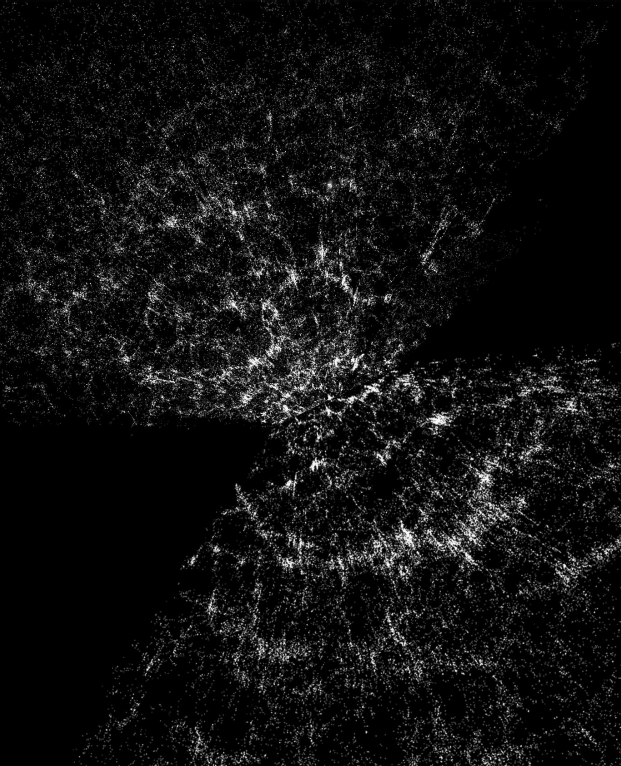
\includegraphics[scale = 0.65]{sdss_redshift}
	\caption{SDSS is the largest and most systematic sky survey in the history of astronomy. It is a combination of a sky survey in 5 optical bands of 25\% of the celestial (northern) sphere. Each image is recorded on CCDs in these 5 bands. On the basis of the images/colours and their brightness a million galaxies are subsequently selected for spectroscopic follow-up. The total sky area covered by SDSS is 8452 square degrees. This image is taken from a movie made by Subbarao, Surendran and Landsberg (see website: \url{https://astro.uchicago.edu/research/cosmus.php}). It depicts the resulting redshift distribution after the 3rd public data release. It concerns 5282 square degrees and contained 528,640 spectra, of which 374,767 galaxies \citep{van_de_weygaert_cosmic_2011}.}
	\label{fig:sdss_rdshft}
\end{figure}
\begin{figure}
	\centering
	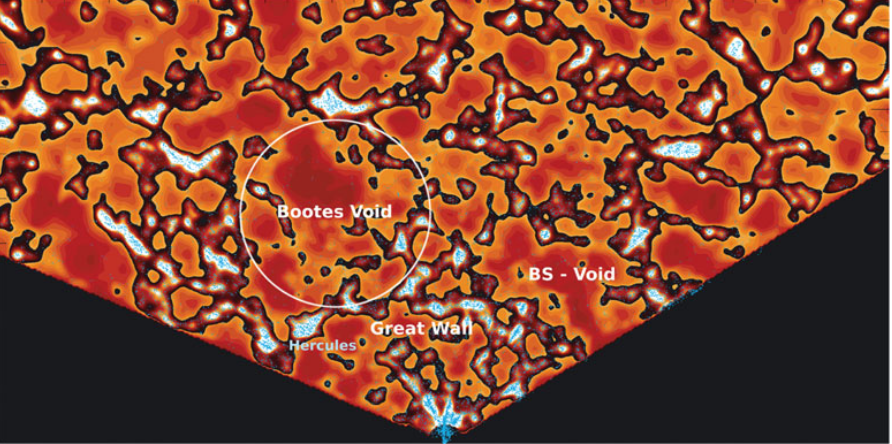
\includegraphics[scale=0.37]{sdss_bootes}
	\caption{SDSS density map and galaxies in the a region of the SDSS galaxy redshift survey region containing the canonical Bo\"{o}tes void. The galaxies in the SDSS survey are superimposed as dark dots. The underdense voids are clearly outlined as the lighter region outside the high-density weblike filamentary and wall-like features \citep{van_de_weygaert_voids_2014}.}
	\label{fig:sdss_bootes}
\end{figure}


The insights aided by surveying projects like the 2dF (Two-degree field ) Galaxy Redshift Survey \citep{colless_2df_2001} and the Sloan Digital Sky Survey \citep{tegmark_threedimensional_2004} building upon early galaxy redshift surveys \citep{chincarini_size_1975, gregory_perseuspisces_1978, zeldovich_giant_1982} established voids as an integral component of the cosmic web. With further developments, it has now been realized that voids not only represent an integral part of the cosmic web but also act as excellent probes and measures of global cosmology \citep{van_de_weygaert_voids_2014}. 

Voids contain a considerable amount of information on the underlying cosmological scenario and on global cosmological parameters. Notable cosmological imprints are found in the outflow velocities and accompanying redshift distortions \citep{martel_simulation_1990, dekel_omega_1994, ryden_voids_1996}. The pristine low-density environment of voids represents an ideal and pure setting for the study of galaxy formation and the influence of cosmic environment on the formation of galaxies \citep{kreckel_only_2011, kreckel_void_2012}. Furthermore, voids have also been believed to have played a prominent role in the reionization process in the early Universe \citep{furlanetto_cosmology_2006, morales_reionization_2010}.

In this review of these crucial features of the cosmic web, we will start with building the foundations of cosmology and will explore how large-scale structures of the Universe can be quantitatively described. After that, we will build upon the existing reviews \citep{van_de_weygaert_cosmic_2011, van_de_weygaert_voids_2014} to understand the formation, evolution and dynamics of voids and will comment on their current state of research by discussing theoretical models and how they complement to observations. We will also explore the void galaxies, the lonesome galaxies located in the voids, as they provide key constraints on our understanding of galaxy formation in a cosmological context \citep{kreckel_void_2014}. We will also discuss the discourses the study of cosmic voids has transpired in broader domains of cosmology relating to dark energy and the standard cosmological model. In the end, after contemplating the results, we will discuss the future of the research in this field.
%This is a simple template for authors to write new MNRAS papers.
%See \texttt{mnras\_sample.tex} for a more complex example, and \texttt{mnras\_guide.tex}
%for a full user guide.
%
%All papers should start with an Introduction section, which sets the work
%in context, cites relevant earlier studies in the field by \citet{Fournier1901},
%and describes the problem the authors aim to solve \citep[e.g.][]{vanDijk1902}.
%Multiple citations can be joined in a simple way like \citet{deLaguarde1903, delaGuarde1904}.

\section{The Large-scale Universe}
In order to formally study large-scale structures of the Universe like cosmological voids, it is essential to be well-versed through fundamentals of physical cosmology. In this section, we will lay the foundations that trace their origins all the way back to Einstein's theory of general relativity and will develop techniques that enable us to quantitatively describe the large-scale Universe. 
%Normally the next section describes the techniques the authors used.
%It is frequently split into subsections, such as Section~\ref{sec:maths} below.

\subsection{The Friedmann Equations}
In 1922, using Einstein's field equations of gravitation for the Friedmann–Lema\^{i}tre–Robertson–Walker metric and a perfect fluid with a given mass density $ \rho $ and pressure $ p $, Alexander Friedmann derived his equations that govern the expansion of space in homogeneous and isotropic models of the universe \citep{friedman_uber_1922}. They are as follows:
\begin{equation}\label{key}
	\dfrac{\dot{a} + kc^2}{a^2} = \dfrac{8 \pi G \rho + \Lambda c^2}{3}
\end{equation}
and
\begin{equation}\label{key}
	\dfrac{\ddot{a}}{a} = -\dfrac{4 \pi G}{3} \Bigg(\rho + \dfrac{3p}{c^2}\Bigg) + \dfrac{\Lambda c^2}{3}
\end{equation}
\label{sec:maths} % used for referring to this section from elsewhere

Here $ a $ is a dimensionless quantity called the scale factor and it is a function of time. The scale factor acts as a parameter which describes the relative expansion rate of the Universe. $ \dot{a} $ and $ \ddot{a} $ are with respect to time. $ k $ is a constant for a particular solution, $ G $ is the Newton's gravitational constant and $ \Lambda $ is the cosmological constant.

These equations lie at the core of every theoretical model in physical cosmology and the evolution of large-scale structures like filaments and voids is described most accurately by them.

\subsection{Distance Measures}
As the Universe is expanding with time, we need a framework to specify the distances between any two points in space at any point in time. This is important when it comes to analytically study large-scale structures of the Universe. The most well-known consequence of expansion of space is the cosmological redshift, defined as the fractional Doppler shift of its emitted light resulting from radial motion \citep{hogg_distance_2000}:
\begin{equation}\label{key}
	z \equiv \dfrac{\nu_e}{\nu_o} - 1 = \dfrac{\lambda_o}{\lambda_e} - 1
\end{equation}
where $ \nu $ is the frequency, $ \lambda $ is the wavelength and subscripts $ e $ and $ o $ denote emitted and observed quantities respectively, 
\textit{Hubble's law} is the observation that all sufficiently distant objects from Earth are moving away from it at speeds proportional to their distances.

There are many ways in which distances in cosmology are defined and they all are asymptotic to each other for small redshifts. Further, it is actually convenient to express these distances as functions of redshift since it is always an observable.

The \textit{comoving distance} is one of the most important distance type and can be contrasted with \textit{proper distance} as the distance which remains constant over cosmological time as it takes account for the expansion of the Universe. It is defined as:
\begin{equation}\label{key}
	d_C (z) = d_H \int_0^z \dfrac{dz'}{E(z')}
\end{equation}
along the line of sight (LOS), where $ d_H $ is the \textit{Hubble distance}, given by $ d_H = c/H_0 \approx \SI{3000}{\per \h \mega \parsec} = \SI{9.26e25}{\per \h \meter} $, $ c $ being speed of light and $ H_0 $ is \textit{Hubble parameter} at the present. The symbol $ h $ is the \textit{dimensionless Hubble constant} and considered a unit itself. The Hubble constant is provides the mathematical form of the Hubble's law as $ H_0 = v/D $ where $ v $ is the velocity of separation and $ D $ is cosmological time-dependent proper distance. Further, we define the \textit{dimensionless Hubble parameter} \citep{peebles_principles_1993}:
\begin{equation}\label{key}
	E (z) = \dfrac{H(z)}{H_0} = \sqrt{\Omega_r (1+z)^4 + \Omega_m (1+z)^3 + \Omega_k(1+z)^2 + \Omega_{\Lambda}}
\end{equation}
Here, $ \Omega_{r} $, $ \Omega_{m} $ and $ \Omega_{\Lambda} $ are normalized values of the present radiation energy density, matter density, and \textit{dark energy density,} respectively with $ \Omega_k = 1 - \Omega_{r} - \Omega_{m} - \Omega_{\Lambda}$ determining the curvature. 

In due course, we will see that catalogs courtesy of sky surveying projects like the \textit{Sloan Digital Sky Survey} (SDSS) often report distances related to large scale-structures like voids in form of comoving distance so it is necessary to understand this development. The theory of Friedmann equations and different distances forms the theoretical aspect of cataloging any large-scale structure in the Universe, with observations gathered from the sky surveying projects using ground based telescopes and even in space probes (like with the \textit{Planck} project for detecting cosmic microwave background anisotropies).


\section{Formation, Evolution and Dynamics of Voids}

\begin{equation}
	\dfrac{d^2 \mathcal{R}_\textrm{m}}{dt^2} = -4 \pi G \rho_u (t) \Bigg[\dfrac{1+\delta}{3} + \dfrac{1}{2}\Big(\alpha_m - \dfrac{2}{3} \Big)\delta \Bigg] \mathcal{R}_\textrm{m} - \tau_\textrm{m} \mathcal{R}_\textrm{m} + \Lambda R_m
\end{equation}

\subsection{Void Dyanmics}
\subsubsection{The Homegenous Ellipsodidal Model}
\subsection{Void Sociology}


\section{Void Galaxies}
\section{Results}
\section{Discussions}
\section{Conclusions}
\section*{Acknowledgements}

The Acknowledgements section is not numbered. Here you can thank helpful
colleagues, acknowledge funding agencies, telescopes and facilities used etc.
Try to keep it short.

%%%%%%%%%%%%%%%%%%%%%%%%%%%%%%%%%%%%%%%%%%%%%%%%%%
\section*{Data Availability}

 
The inclusion of a Data Availability Statement is a requirement for articles published in MNRAS. Data Availability Statements provide a standardised format for readers to understand the availability of data underlying the research results described in the article. The statement may refer to original data generated in the course of the study or to third-party data analysed in the article. The statement should describe and provide means of access, where possible, by linking to the data or providing the required accession numbers for the relevant databases or DOIs.




%%%%%%%%%%%%%%%%%%%% REFERENCES %%%%%%%%%%%%%%%%%%

% The best way to enter references is to use BibTeX:
\bibliographystyle{mnras}
\bibliography{p463} % if your bibtex file is called example.bib


% Alternatively you could enter them by hand, like this:
% This method is tedious and prone to error if you have lots of references
%\begin{thebibliography}{99}
%\bibitem[\protect\citeauthoryear{Author}{2012}]{Author2012}
%Author A.~N., 2013, Journal of Improbable Astronomy, 1, 1
%\bibitem[\protect\citeauthoryear{Others}{2013}]{Others2013}
%Others S., 2012, Journal of Interesting Stuff, 17, 198
%\end{thebibliography}

%%%%%%%%%%%%%%%%%%%%%%%%%%%%%%%%%%%%%%%%%%%%%%%%%%

%%%%%%%%%%%%%%%%% APPENDICES %%%%%%%%%%%%%%%%%%%%%

\appendix

\section{Some extra material}

If you want to present additional material which would interrupt the flow of the main paper,
it can be placed in an Appendix which appears after the list of references.

%%%%%%%%%%%%%%%%%%%%%%%%%%%%%%%%%%%%%%%%%%%%%%%%%%


% Don't change these lines
%\bsp	% typesetting comment
\label{lastpage}
\end{document}

% End of mnras_template.tex
